% expression_chain.tex — one model of expression, three depths of measurement
\documentclass[tikz,border=10pt]{standalone}
\usetikzlibrary{positioning,arrows.meta,fit}
\definecolor{ink}{HTML}{1A1A1A}
\definecolor{muted}{HTML}{6B7280}
\definecolor{okblue}{HTML}{0072B2}
\definecolor{okamber}{HTML}{E69F00}
\definecolor{okverm}{HTML}{D55E00}
\definecolor{okgreen}{HTML}{009E73}
\begin{document}
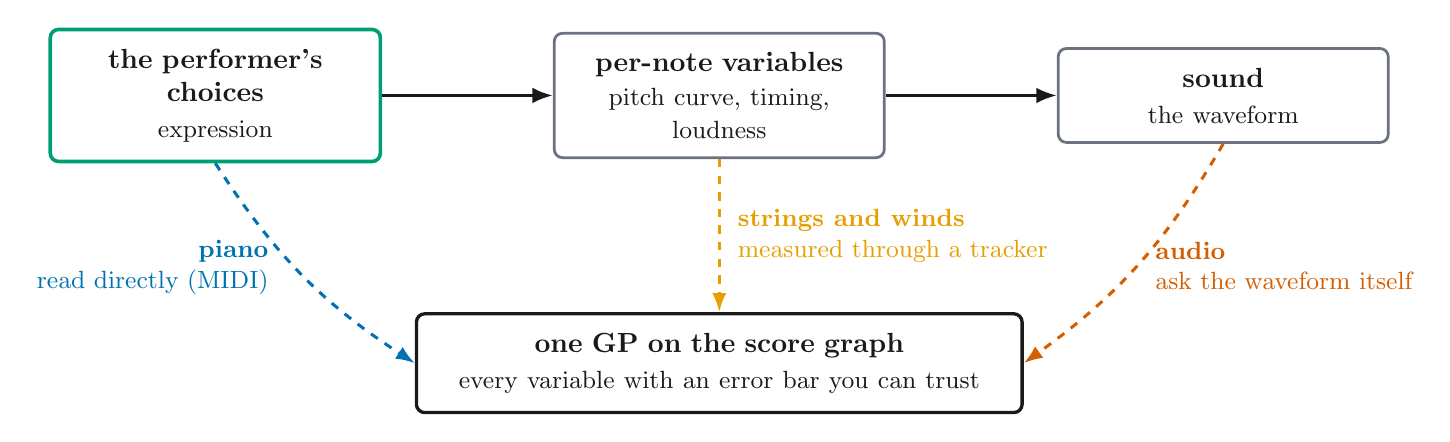
\begin{tikzpicture}[font=\normalsize,
  n/.style={draw=muted, line width=1pt, rounded corners=3pt, fill=white,
            align=center, inner sep=7pt, text width=37mm, text=ink},
  arr/.style={-{Latex[length=2.6mm,width=2mm]}, draw=ink, line width=1.1pt},
  tap/.style={-{Latex[length=2.4mm,width=1.8mm]}, line width=1.1pt, dashed},
]
\node[n, draw=okgreen, line width=1.3pt] (E) at (0, 0)
  {\textbf{the performer's}\\ \textbf{choices}\\[1pt] \small expression};
\node[n] (C) at (6.4, 0)
  {\textbf{per-note variables}\\[1pt] \small pitch curve, timing,\\ \small loudness};
\node[n] (S) at (12.8, 0)
  {\textbf{sound}\\[1pt] \small the waveform};
\draw[arr] (E) -- (C);
\draw[arr] (C) -- (S);
\node[n, draw=ink, line width=1.2pt, text width=72mm] (M) at (6.4, -3.4)
  {\textbf{one GP on the score graph}\\[1pt]
   \small every variable with an error bar you can trust};
\draw[tap, okblue] (E.south) to[bend right=12]
  node[left, font=\small, text=okblue, align=right, xshift=-3mm, yshift=1mm]
  {\textbf{piano}\\ read directly (MIDI)} (M.west);
\draw[tap, okamber] (C.south) --
  node[right, font=\small, text=okamber, align=left, xshift=1mm]
  {\textbf{strings and winds}\\ measured through a tracker} (M.north);
\draw[tap, okverm] (S.south) to[bend left=12]
  node[right, font=\small, text=okverm, align=left, xshift=1mm]
  {\textbf{audio}\\ ask the waveform itself} (M.east);
\end{tikzpicture}
\end{document}
